\chapter{Fault  analysis}
\textit{In this chapter, probable faults in the system are examined using a Failure Mode and Effects Analysis (FMEA). Next, in order to find how probable a fault will happen and the effect of it, the severity and occurrance (SO) of faults is analyzed. It was decided that the fault analysis will be carry out only for the actuators (magnetorquers and momentum wheels).}

A fault in a system can be seen as a sudden shift in the system functionality, nevertheless, it might not mean a total shutdown of the system. One way to see it is as a disturbance in the system, that might cause performance loss or serious deterioration to the system. On the other hand, a failure can be understood as a total shutdown of the system component. 

In \figref{fig:1} a fault tolerant system is described, which contains an autonomous supervisor that has the ability to switch between various controllers taking into account the type of fault that a component has. The spacecraft block illustrated in the picture is composed of a plant, actuators and sensors and is monitored by the fault detection and isolation (FDI) system, which include detectors that will feed informations to the supervisor in the eventuality of a fault. Based on the information received, the supervisor will establish if a fault occurred or not and in case of a fault the effectors will handle it. Figure \ref{fig:2} shows the procedure of how faults are handled with varius methods.

\begin{table}[H]
	\begin{minipage}[b]{0.49\linewidth}
		\centering
		\begin{figure}[H]
			\centering
			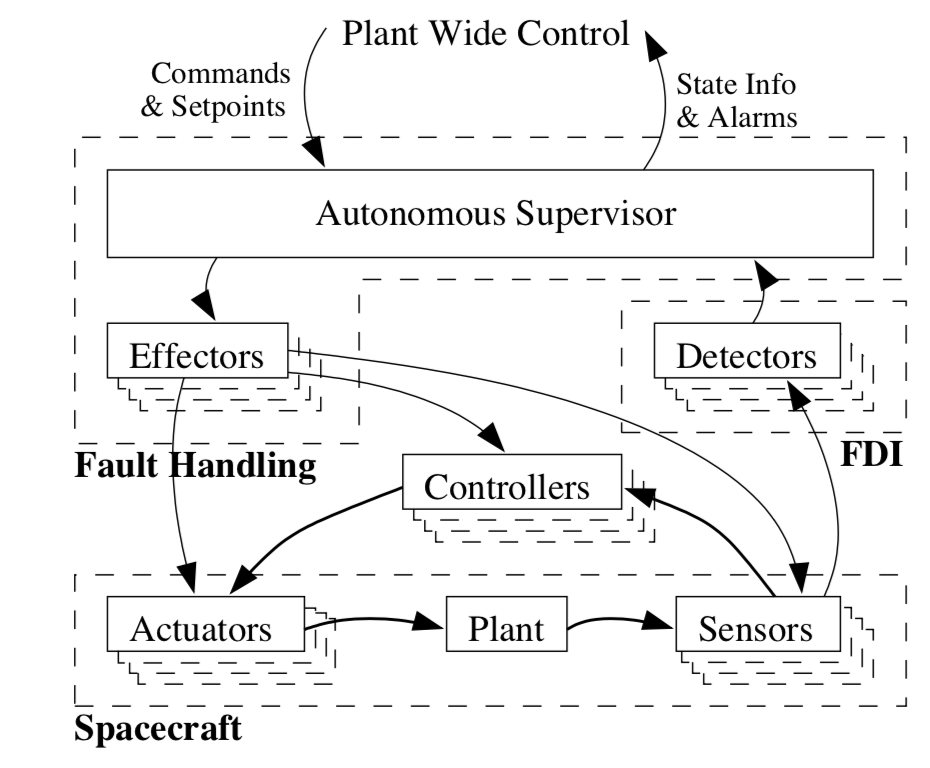
\includegraphics[width=1\linewidth]{figures/FTC}
			\caption{Fault tolerant system architecture [ref jesper article}
			\label{fig:1}
		\end{figure}
	\end{minipage}\hfill
	\begin{minipage}[b]{0.49\linewidth}
		\centering
		\begin{figure}[H]
			\centering
			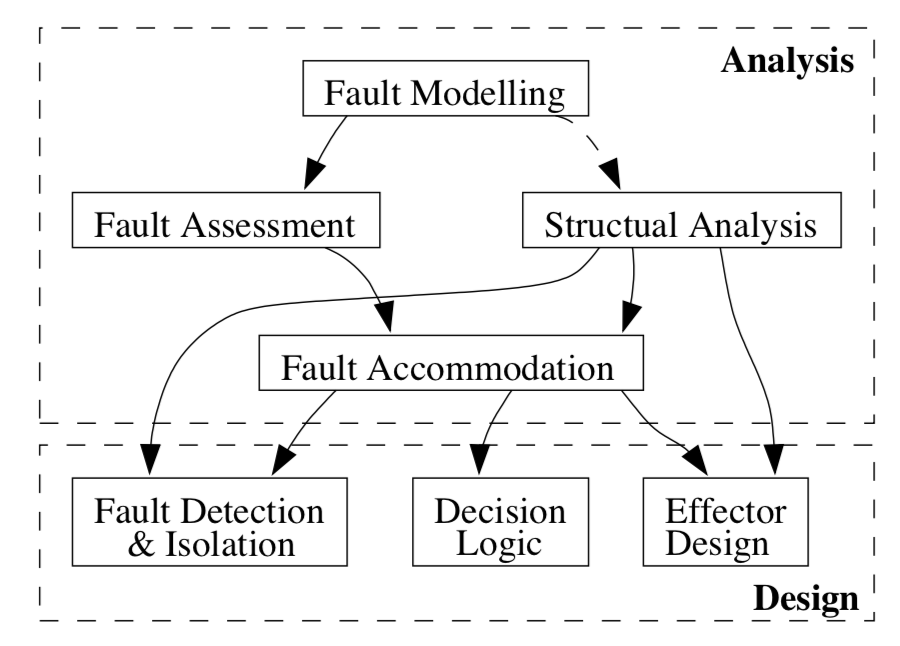
\includegraphics[width=1\linewidth]{figures/FTC_2}
			\caption{ }
			\label{fig:2}
		\end{figure}
	\end{minipage}
\end{table}

\subsection{Failure Mode and Effects Analysis}
A FMEA analysis which is a bottom-up analysis method is performed for the components of the satellite. The main goal of FMEA is to identify possible faults and their effects on components. In order to evaluate how faults are propagated through the system, a FMEA scheme is constructed.
Another aspect of FMEA analysis is that, the severity of a fault can be determined, which will offer the opportunity to prioritize the faults by severity and in this way focus on the important faults.

In order to control the attitude of the satellite, two types of actuators are used: magnetorquers and momentum wheels. Potential faults are gather into a table which describes the effect and cause, while the satellite is orbiting.
\subsubsection{Magnetorquers}

\begin{table}[H]
	\centering
	\label{my-label}
	\begin{tabular}{|l|l|l|}
		\hline
		\multicolumn{3}{|c|}{\textit{\textbf{Magnetorquers}}}                                          \\ \hline
		\multicolumn{3}{|c|}{Produces a magnetic field that interacts with Earth's magnetic field}                     \\ \hline
		\textbf{Reference} & \textbf{Failure Effect} & \textbf{Failure Cause}                          \\ \hline
		$MT_1$                 & Low magnetic field  & \begin{tabular}[c]{@{}l@{}}- Broken wire or bad soldering\\ - Component burned\end{tabular} \\ \hline
		$MT_2$                 & Maximum magnetic field power  & Short circuit to the power voltage   \\ \hline
		$MT_3$                 & Wrong direction of the magnetic field & \begin{tabular}[c]{@{}l@{}}- Misalignment of the magnetorquer\\ - Short circuit of some parts of the \\ torquer to the power voltage \end{tabular} \\ \hline
		$MT_4$                 & Wrong  power of the magnetic field                 & Floating supplay voltage                                            \\ \hline
	\end{tabular}
	\caption{Potential faults in the magnetorquers}
\end{table}

\subsubsection{Momentum wheels}

\begin{table}[H]
	\centering
	\label{my-label}
	\begin{tabular}{|l|l|l|}
		\hline
		\multicolumn{3}{|c|}{\textit{\textbf{Momentum wheels}}}                                          \\ \hline
		\multicolumn{3}{|c|}{Produces a torque about the satellite COM in order to rotate it }                     \\ \hline
		\textbf{Reference} & \textbf{Failure Effect} & \textbf{Failure Cause}                          \\ \hline
		$MW_1$                & Faulty orientation/alter the angular velocity & \begin{tabular}[c]{@{}l@{}} Shifting of the flywheel \\throughout launch or transport \\   \end{tabular} \\ \hline
		$MW_2$                & Unable to control the rotation   & A difference in the power voltage  \\ \hline
		$MW_3$                & No torque received& \begin{tabular}[c]{@{}l@{}} Short circuit to the ground\\  \end{tabular} \\ \hline
		$MW_4$                & Increased rotations of the flywheel  & Broken wire or bad soldering                                          \\ \hline
	\end{tabular}
	\caption{Potential faults in the momentum wheels}
\end{table}
\subsubsection{Severity and occurrence evaluation}
To investigate the faults that have the biggest rate of occurrence, the severity of the effects of failures and the probability of occurrence is determined based on the faults from FMEA. This procedure describes how to each fault receives a severity index (SO) and an occurrence index(OI). A table containing the serverity and occurrence for magnetorquers is shown as follows:
\begin{table}[H]
	\centering
	\label{11}
	\begin{tabular}{|l|l|l|l|}
		\hline
		\multicolumn{4}{|c|}{\textit{Magnetorquer}}                                                                                         \\ \hline
		Reference & Severity & Occurrence                                          & SO Index                                      \\ \hline
		$MT_1$     & 7        & \begin{tabular}[c]{@{}l@{}}- 5\\ - 4\end{tabular} & \begin{tabular}[c]{@{}l@{}}- 35\\- 28\end{tabular} \\ \hline
		$MT_2$       & 10       & 3       & 30                \\ \hline
		$MT_3$       & 3        & \begin{tabular}[c]{@{}l@{}}- 2\\- 1\end{tabular} & \begin{tabular}[c]{@{}l@{}}- 6\\- 3\end{tabular} \\ \hline
		$MT_4$       & 4        & 6                   & 24                  \\ \hline
	\end{tabular}
\caption{SO for magnetorquer}
\end{table}
The same procedure is done for momentum wheels as follows:
\begin{table}[H]
	\centering
	\label{12}
	\begin{tabular}{|l|l|l|l|}
		\hline
		\multicolumn{4}{|c|}{\textit{Momentum wheels}}                                                                                         \\ \hline
		Reference & Severity & Occurrence                                          & SO Index                                      \\ \hline
		$MW_1$      & 1        & \begin{tabular}[c]{@{}l@{}}7\\ \end{tabular} & \begin{tabular}[c]{@{}l@{}}7\\ \end{tabular} \\ \hline
		$MW_2$        & 1        & 4             & 4                                         \\ \hline
		$MW_3$        & 2        & \begin{tabular}[c]{@{}l@{}}3\\\end{tabular} & \begin{tabular}[c]{@{}l@{}}8\\ \end{tabular} \\ \hline
		$MW_4$        & 4        & 2     & 8               \\ \hline
	\end{tabular}
	\caption{SO for momentum wheels}
\end{table}

The severity index is computed using the following formula:
\begin{flalign}
	SO_{index} = severity \cdot occurrence
	\label{eq:ec1}
\end{flalign} 

\subsubsection{Fault propagation analysis}
In order to observe how faults are propagated through the system and the effect of these faults, a FMEA scheme is constructed. Further computation will be on the appendix.
\subsection{Fault detection and isolation}


\chapter{Attitude control}
\section{Modelling}
This section describes the mathematical model of the satellite which contains the dynamic and kinematic model, based on the rigid body dynamics and kinematics.
\subsection{Spacecraft dynamic equation}
The satellite dynamics are described using Euler's equation of motion and Newton's laws of motion. 
Using Euler's equation of motion, the relation between the change in angular momentum and the torques that affect the satellite is given as follows:
\begin{flalign}
	\vec{ \dot h} = \vec{N_{ext}} =  \vec{N_{mt}}+ \vec{N_{dist}}
	\label{eq:ec2}
\end{flalign} 
where $h$ is the angular momentum of a rigid body, $N_{ext}$ represent all the external torques that influence the satellite, $N_{mt}$ is the torque from the magnetorquers and $N_{dist}$ is the torque from the disturbances.

The change in angular momentum of the satellite can be express as the product between the angular acceleration and the moment of inertia:
\begin{flalign}
	{\vec{\dot h_{sat}}} = {\underline I_{s}}{\vec{\dot \omega}}
	\label{eq:ec3}
\end{flalign} 
where $h_{sat}$ is the angular momentum of the satellite, $\underline I_{s}$ is the moment of inertia of the satellite and $\vec{\omega}$ is the angular velocity.

Including the momentum wheels, the total angular momentum is given by:
\begin{flalign}
	{\vec{h_{tot}}} = \vec{h_{sat}} + \vec{h_{mw}}
	\label{eq:ec4}
\end{flalign} 
where $\vec{h_{mw}}$ is the angular momentum of the momentum wheels.
Therefore, the total angular momentum is described by:
\begin{flalign}
	{\vec{h_{tot}}} = {\underline I_{s}}{\vec{\omega}}+{\vec{h_{mw}}}
	\label{eq:ec5}
\end{flalign}
By rearranging terms, equation \ref{eq:ec5} becomes:
\begin{flalign}
	{\vec{\omega}} = {\underline I_{s}^{-1}} ({\vec{h_{tot}}}-{\vec{h_{mw}}})
	\label{eq:ec6}
\end{flalign}

Using Euler's equation of motion, the time derivative of $\vec{h_{tot}}$ expressed in the ECI frame is:\todo{maybe a more thorough description of the 1st eq like in witch frame is described}
\begin{flalign}
	&	\vec{ \dot h_{tot}} = \vec{ \dot h_{sat}} + \vec \omega \times \vec h= \vec{  N_{mt}} + \vec{  N_{dist}} \\
	 &\underline I_s {\vec{\dot{\omega}}} + \vec {\dot{h}_{rw}}+ \vec \omega \times \vec L = \vec{  N_{mt}} + \vec{  N_{dist}} 
	 \label{eq:ec7}
 \end{flalign}
Subsequently, the angular velocity is separtated and expressed as:
\begin{flalign}
{\vec{\dot{\omega}}} = -\underline I_s ^{-1} \vec \omega \times \vec L -\underline I_s ^{-1} \vec {\dot{h}_{mw}} + \underline I_s ^{-1}(\vec{  N_{mt}} + \vec{  N_{dist}}) 
\label{eq:ec8}
\end{flalign}
Next, by replacing the cross product with a skew-symmetric matrix ${\underline S(\vec \omega)}$, \eqref{eq:ec8} becomes:
\begin{flalign}&{\vec{\dot{\omega}}}={-\underline I_{s}^{-1}\underline S(\vec \omega)\underline I_{s}\vec \omega-\underline I_{s}^{-1}\underline S(\vec \omega)\vec h_{mw}-\underline I_s ^{-1}\vec{  N_{mw}} + \underline I_s ^{-1}(\vec{  N_{mt}} + \vec{  N_{dist}})}
\label{eq:ec9}
\end{flalign}
where $N_{mt}$ is the torque from the magnetorquers, $N_{mw}$ is the torque from the momentum wheels and the skew-symmetric matrix is:
\begin{flalign}
	{\underline S(\vec \omega)}
	= 
	\begin{bmatrix}
		0& -\omega_{3}& \omega_{2} \\
		\omega_{3}& 0&-\omega_{1}  \\ 
		-\omega_{2} & \omega_{1} &0
	\end{bmatrix} 
	\label{eq:skewsymmetricmatrix}
\end{flalign}
Moreover, the torque set to the momentum wheels is equal to the time derivative of the angular momentum:
\begin{flalign}
    \vec {N_{mw}} =  {\vec{ \dot{h}_{mv}}}
	\label{eq:ec10}
\end{flalign}
\subsection{Spacecraft kinematic equation}
In this subsection, the focus will be on describing the orientation of the satellite. The method used for describing the satellite attitude is quaternion representation. It was decided to choose quaternion representation, because they provide a way to deal with singularities.

The quaternion $\textbf{q}(t)$ is defined as the attitude quaternion of a rigid body at time $t$ with respect to the inertial frame and at time $t+\Delta t$, the quaternion $\textbf{q}(t+\Delta t)$ is defined. The orientation quaternion can be divided into the quaternion at time $t$ and performing a quaternion multiplication with the rotation in the interval $\Delta t$ as follows:
\begin{flalign}
	\vec{ ^s_iq}(t+\Delta{t}) = \vec{ q}(\Delta {t}) \otimes \vec{ ^s_i q}(t) 
	\label{eq:qp}
\end{flalign}
where the orientation quaternion $	\vec{ ^s_iq}(t+\Delta{t}) $ represents the rotation of the spacecraft body frame with respect to the intertial frame

The quaternion at time $\Delta t$ can be express using the triad $u, v, w$, that represent the axis of the spacecraft as:
%
\begin{flalign}
	q_{1}(\Delta {t})  = {e_{u}\sin\frac{\Delta\Phi}{2}}
	\label{eq:q11}
\end{flalign}
%
\begin{flalign}
	q_{2}(\Delta {t}) = {e_{v}\sin\frac{\Delta\Phi}{2}}
	\label{eq:q2}
\end{flalign}
%
\begin{flalign}
	q_{3} (\Delta {t})= {e_{w}\sin\frac{\Delta\Phi}{2}}
	\label{eq:q3}
\end{flalign}
%
\begin{flalign}
	q_{4}(\Delta {t}) = {\cos\frac{\Delta\Phi}{2}}
	\label{eq:q4}
\end{flalign}
where $\Delta \Phi$ is the rotation at time $\Delta t$ and $e_u,e_v, e_w$ are the components along the triad $u, v, w$ at time $\Delta t$.

Using equation \ref{eq:q11} and equation \ref{eq:q4} and insert them into equation \ref{eq:qp} which yields:
\begin{flalign}
	\vec{ ^s_i q}(t+\Delta{t})
	= 
	\left\{\cos\frac{\Delta\Phi}{2} \underline I_{(4\times4)}+\sin\frac{\Delta\Phi}{2}
	\begin{bmatrix}
		0 &e_{z}&-e_{y}&e_{x} \\
		-e_{z}&0&e_{x}&e_{y}  \\ 
		e_{y}&-e_{x}&0&e_{z} \\
		-e_{x} &e_{y}&-e_{z}&0
	\end{bmatrix} 
	\right \} \vec{ ^s_i q}(t)
	\label{eq:quatm}
\end{flalign}  
%
where $\underline I$ is the identity matrix with the dimensions of $4\times4$.

In order to turn equation \ref{eq:quatm} into a differential equation, a small angle approximation it is used: 
\begin{flalign}
	&\Delta \phi = \omega \ \Delta t \\
	&\cos\frac{\Delta\Phi}{2} \approx 1 \\	
	&\sin\frac{\Delta\Phi}{2} \approx \frac{\omega \Delta t }{2} \\
	\label{eq:aprox}
\end{flalign} 
After using the approximation and substitute the terms into \ref{eq:quatm}, the following equation is obtained:
\begin{flalign}
	\vec{^s_i q(t+\Delta{t})} \approx \left[1 + \frac{1}{2} \underline \Omega \Delta(t)\right]\vec{^s_i q(t)}
	\label{eq:quatfinal}
\end{flalign} 
where $\underline \Omega$ is the skew symmetric matrix written in form:
\begin{flalign}
	\underline \Omega
	= 
	\begin{bmatrix}
		0& \omega_{w}& - \omega_{v}& \omega_{u} \\
		-\omega_{w}& 0&\omega_{u}& \omega_{v}  \\ 
		\omega_{v}& -\omega_{u}&0& \omega_{w} \\
		-\omega_{u}& -\omega_{v}& -\omega_{w}&0
	\end{bmatrix} 
	\label{eq:sm}
\end{flalign}
where the terms $\omega_u, \omega_v, \omega_w$ are the angular velocities.

The rate of change in the orientation of the spacecraft $\vec{^s_i q(t)}$  can be found:
\begin{flalign}
	\vec{ ^s_i\dot q(t)} = \lim_{\Delta t\to 0} \frac{\vec q(t+\Delta t) - \vec q(t)}{\Delta t} = \dfrac{1}{2} \underline \Omega \  \vec{^s_i q(t)}
	\label{eq:finaleq}
\end{flalign} 
\subsection{Spacecraft equation of motion }
Putting together both dynamic and kinematic equation for the spacecraft, the system equations can be combined into a state-space representation:
\begin{flalign}
	\begin{bmatrix}
		\vec{ ^s_i\dot q(t)} \\
		\vec{\dot \omega{(t)}}
	\end{bmatrix} 	
	= 
	\begin{bmatrix}
		\frac{1}{2} \underline{ \Omega}_{(4\times4)} \vec{ ^s_i q(t)} \\
		{-\underline{I}_{s}^{-1}\underline{S}(\vec{\omega})\underline{I}_{s}\vec{\omega}(t)-\underline{I}_{s}^{-1}\underline{S}(\vec{\omega})\vec{h_{mw}}-\underline{I}_{s}^{-1}\vec{N_{mw}}(t)+\underline{I}_{s}^{-1}[\vec{N_{mt}(t)}+\vec{N_{dis}}(t)}]
	\end{bmatrix} 
	\label{eq:seom}
\end{flalign}
where,\\
$\vec{ ^s_i  q(t)} = [q_1 \ q_2 \ q_3 \ q_4]^T$ \\
$\vec{\omega{(t)}} = [ \omega_1 \ \omega_2 \ \omega_3]^T$ \\
$\underline{\Omega}(\omega)$ is the $4\times4$ skew symmetric matrix \\
$\underline{I}_{s}$ is the inertia matrix \\
$\underline{S}(\omega)$ is the $3\times3$ skew symmetric matrix \\
$\vec{N_{dis}}(t)$ is the disturbance torque \\
$\vec{N_{mw}}$ is the torque from momentum wheels \\
$\vec{N_{mt}}$ is the torque from magnetorquers  \\